\documentclass[12pt]{article}
\usepackage{blindtext}
\usepackage[T1]{fontenc}
\usepackage[utf8]{inputenc}
\usepackage[left=1in,top=1in,right=1in,bottom=1in]{geometry} 
\usepackage{hyperref}
\usepackage{titlesec}
\titlespacing\section{0pt}{12pt plus 2pt minus 2pt}{0pt plus 1pt minus 1pt}
\usepackage{endnotes}
\usepackage{setspace}
\usepackage{graphicx}
\usepackage{fancyhdr}
\pagestyle{fancy}
\fancyhead[L]{\textit{REDJABOEV}}
\fancyhead[R]{\textit{Women in Autocratic Ruling Families}}
\renewcommand{\headrulewidth}{2pt}

\begin{document}

\begin{titlepage}
\centering

\title{Does a Female Relative in Authoritarian Family Improve Women's Outcomes?} 
\author{\textbf{Author:} Khasan Redjaboev\footnote{PhD Student, Department of Political Science, University of Wisconsin–Madison, 110 North Hall, 1050 Bascom Mall, Madison, WI 53706. Email: redjaboev@wisc.edu. This is an edited version of my single-authored original work under development, which was first presented at the PS948 Democratic Imperfections course.}\\
\textbf{Final Project for PS813/PS811} 
\\* \textbf{Professor:} David Weimer
\\* \textbf{Lecturer:} Michael DeCrescenzo
\\* \textbf{Classes:} PS813 Multivariate Statistics and PS811 Computational Statistics}
\date{6 May 2020}
\end{titlepage}

\maketitle


\newpage
\doublespacing

\section*{Question and Motivation}
\textbf{What is the effect of having politically active female members in ruling families of non-democratic\footnote{In this paper, I use the terms ``non-democratic" and ``authoritarian" interchangeably.} countries on pro-feminist policies?} Although imperfect, democracies create better opportunities for both descriptive and substantial representation (Pitkin 1967; Urbinati and Warren 2008). Pitkin (1967) defines four paradigms of representation, implicitly with democracy in mind: formalistic, symbolic, descriptive, and substantive. In authoritarian states, having women\footnote{In this paper, I use the terms ``females" and ``women" interchangeably.} in the positions of power may satisfy one or more of those paradigms, however evaluating authorization (bestowed power legitimacy) and accountability (constituency power to hold accountable) of those women in power is often far from straightforward. Women who get to power or the positions of influence through quasi-governmental links in businesses and NGOs in autocracies are often neither elected nor directly accountable to citizens who they are meant to represent. Therefore, the empirical case validating the mechanisms of accountability in  non-democratic representation is incomplete. Answering this question is important to examining the mechanisms of representation in the absence of democracy. 

In this project, I test if having one or more politically active female family members in an authoritarian ruling family (hereon PAF) can have a positive effect on substantial pro-feminist issues. There are two reasons why this can hold. First, by having a PAF an authoritarian country may seek legitimacy both domestically and internationally (e.g. see Tripp 2019). For example, by increasing symbolic and descriptive representation of women and climbing the international rankings on women's rights. Second, if a PAF delivers substantial pro-feminist policies that may increase women's support by delivering socioeconomic improvements (Aidt and Dallal 2008). Thus, the possibility of these mechanisms benefiting an authoritarian regime warrants a test if ordinary female citizens of non-democracies too \textit{actually} benefit from PAF.   

To conduct this test, I examine the effects of having one or more PAF on pro-feminist legislation and policy outcomes in 69 non-democratic countries across 20 years from 2000 to 2019. All countries ranked in Polity IV as non-democratic twice or more for the given period are included in my panel dataset. This panel set includes all 12 non-Baltic post-Soviet states. Reasoning for the selection (e.g. Ecuador, Moldova, North Korea) or omission of certain countries (e.g. Myanmar) is provided in the \textbf{Data and Empirical Strategy} section. I use the Wikipedia, newspaper, and official profiles of ruling families for 69 selected countries to determine PAF. I use the World Development Indicators databank to measure my covariates and outcomes of interest. The use of panel data is appropriate, because even if there are considerable omissions on states' reporting, cross-country and cross-year variation enables substantial analysis. Panel data is also useful in employing fixed and random effects, henceforth bringing exploratory analysis closer to causal identification. 

\section*{Key Variables of Interest and Hypotheses}
My key independent variable is the presence of politically active female members of ruling families (PAF) in non-democracies. For this research paper, I surveyed Wikipedia profiles of ruling families in 69 countries that were coded as non-democratic in Polity IV dataset in at least two periods out of 20. In addition, at least one reputed newspaper per country of each ruling family and official biographies from governmental websites were researched whenever available. PAF included close relations: mothers, siblings, spouses, and daughters. \texttt{Figure 1} provides a qualitative outlook to all collected profiles. 

%FIGURE 1
\begin{figure}[htp]
\centering
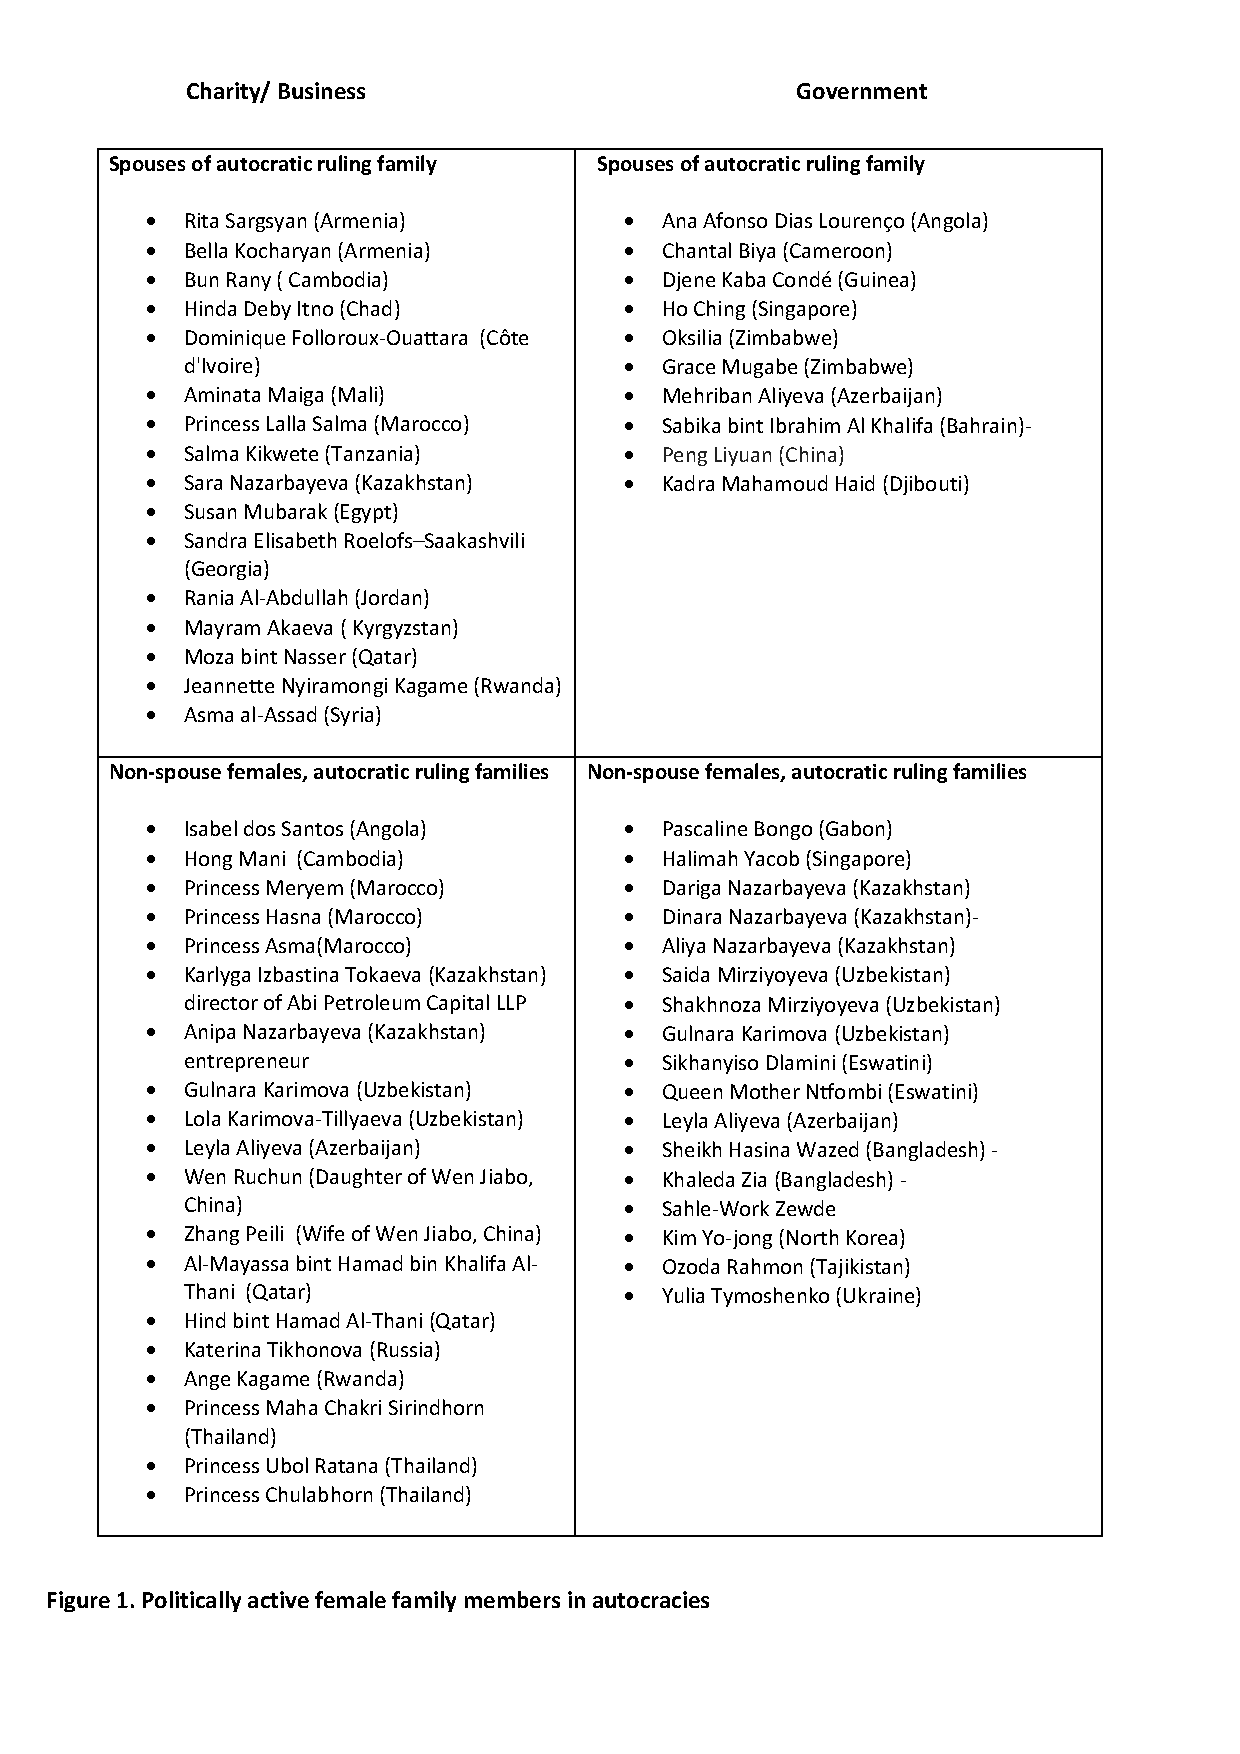
\includegraphics[width=16cm]{Females.pdf}
\label{fig:hypothesis 1 1-2}
\end{figure}

I focus my analysis on families, as family is a starting point in organizational hierarchy of many developing and traditional societies (Cruz et al. 2017:3007). There are several important characteristics that are apparent when examining collected PAF profiles. First, only politically important profiles were collected. To determine if a PAF is likelier to make substantial representation impact, only profiles of a legislator, executive in business with close governmental ties, a state-owned enterprise executive, head of charity or foundation with mandate on public goods and significant governmental funding, a foreign affairs official of senior tier, or governmental or military high tier officials were included. Second, collected profiles were organized in the two by two table by relation to a ruler (spouse and non-spouse) and PAF's occupational profile (charity/business and government). Using the profiles, a binary variable \texttt{female} was created to represent independent variable. Every year when there was one or more PAFs was coded as $1$ for that country and otherwise as $0$.

As can be seen from \texttt{Figure 1}, some profiles appear twice and across columns due to simultaneous presence in both profile roles. For example, Gulnara Karimova, the eldest child of Islam Karimov, late president of Uzbekistan, was at once a businessperson with extensive governmental contracts and a founder of the most influential national non-governmental organization (NGO), and simultaneously an ambassador to European countries and Deputy Minister for Foreign Affairs. There are also profiles of women who are standalone political figures, themselves ruling countries. For example, Sheikh Hasina and Khaleda Zia of Bangladesh were both prime-ministers in the period captured in panel data, period when Bangladesh was coded as non-democratic and with numerous allegations of power abuse from both country leaders. They are placed in the most government column and non-spouse raw. There are some profiles that made transition from one role to another, and thus feature in their most recent roles. Mehriban Aliyeva of Azerbaijan, the spouse of President Ilham Aliyev, and Kim Yo-jong of North Korea, the sibling of Supreme-Leader Kim Jong-un, started in NGO and cultural-symbolic roles, but are currently First Vice-President of Azerbaijan and vice director of the influential Propaganda and Agitation Department, respectively. They are mentioned in the columns that represent their most recent political roles. Other cases are straightforward.

There are two hypotheses advanced by this article. They posit that a presence of PAF in a country is (1) likelier to produce pro-women legislation, but (2) less likely to result in direct policy outcomes. More formally, this can be expressed as: 

HYPOTHESIS 1: \textit{Non-democracies with PAF are likelier to produce pro-women legislation.}

Research on female political participation predicts that women's issues would be better addressed with more women in decision-making roles that have impact on legislation. Will this hold under authoritarianism? I hypothesize that regimes with influential female elites can be better placed to bring about the production of legislative acts that focus on women's issues. Therefore, my dependent variables are seven legislative pieces on women's issues.    

HYPOTHESIS 2: \textit{Non-democracies with PAF will not deliver pro-women policy outcomes.}

This hypothesis is interesting to test, as it involves much more than a cheap-talk by a non-democracy. In line with the theory on authoritarian accountability, I theorize that pro-women laws would not necessarily translate into pro-women policy outcomes. Moreover, important but often overlooked theoretical framework proposed by Pitkin (1967) was based on democratic authorization and accountability. Absent such means, a representative, no matter how descriptively associative and rhetorically substantive, has no incentives to deliver to constituencies. Therefore, my dependent variables are 14 actual pro-women policy outcomes. Rejecting null hypothesis could prove that the presence of PAF can be beneficial, while null effects will be more in line with literature. 

\texttt{Figure 2} provides a summary of all variables used. There are columns for codes, that are the actual variable codes employed in statistical analysis (see R Markdown Appendix) and explanation of each variable's measure. 

%FIGURE 2
\begin{figure}[htp]
\centering
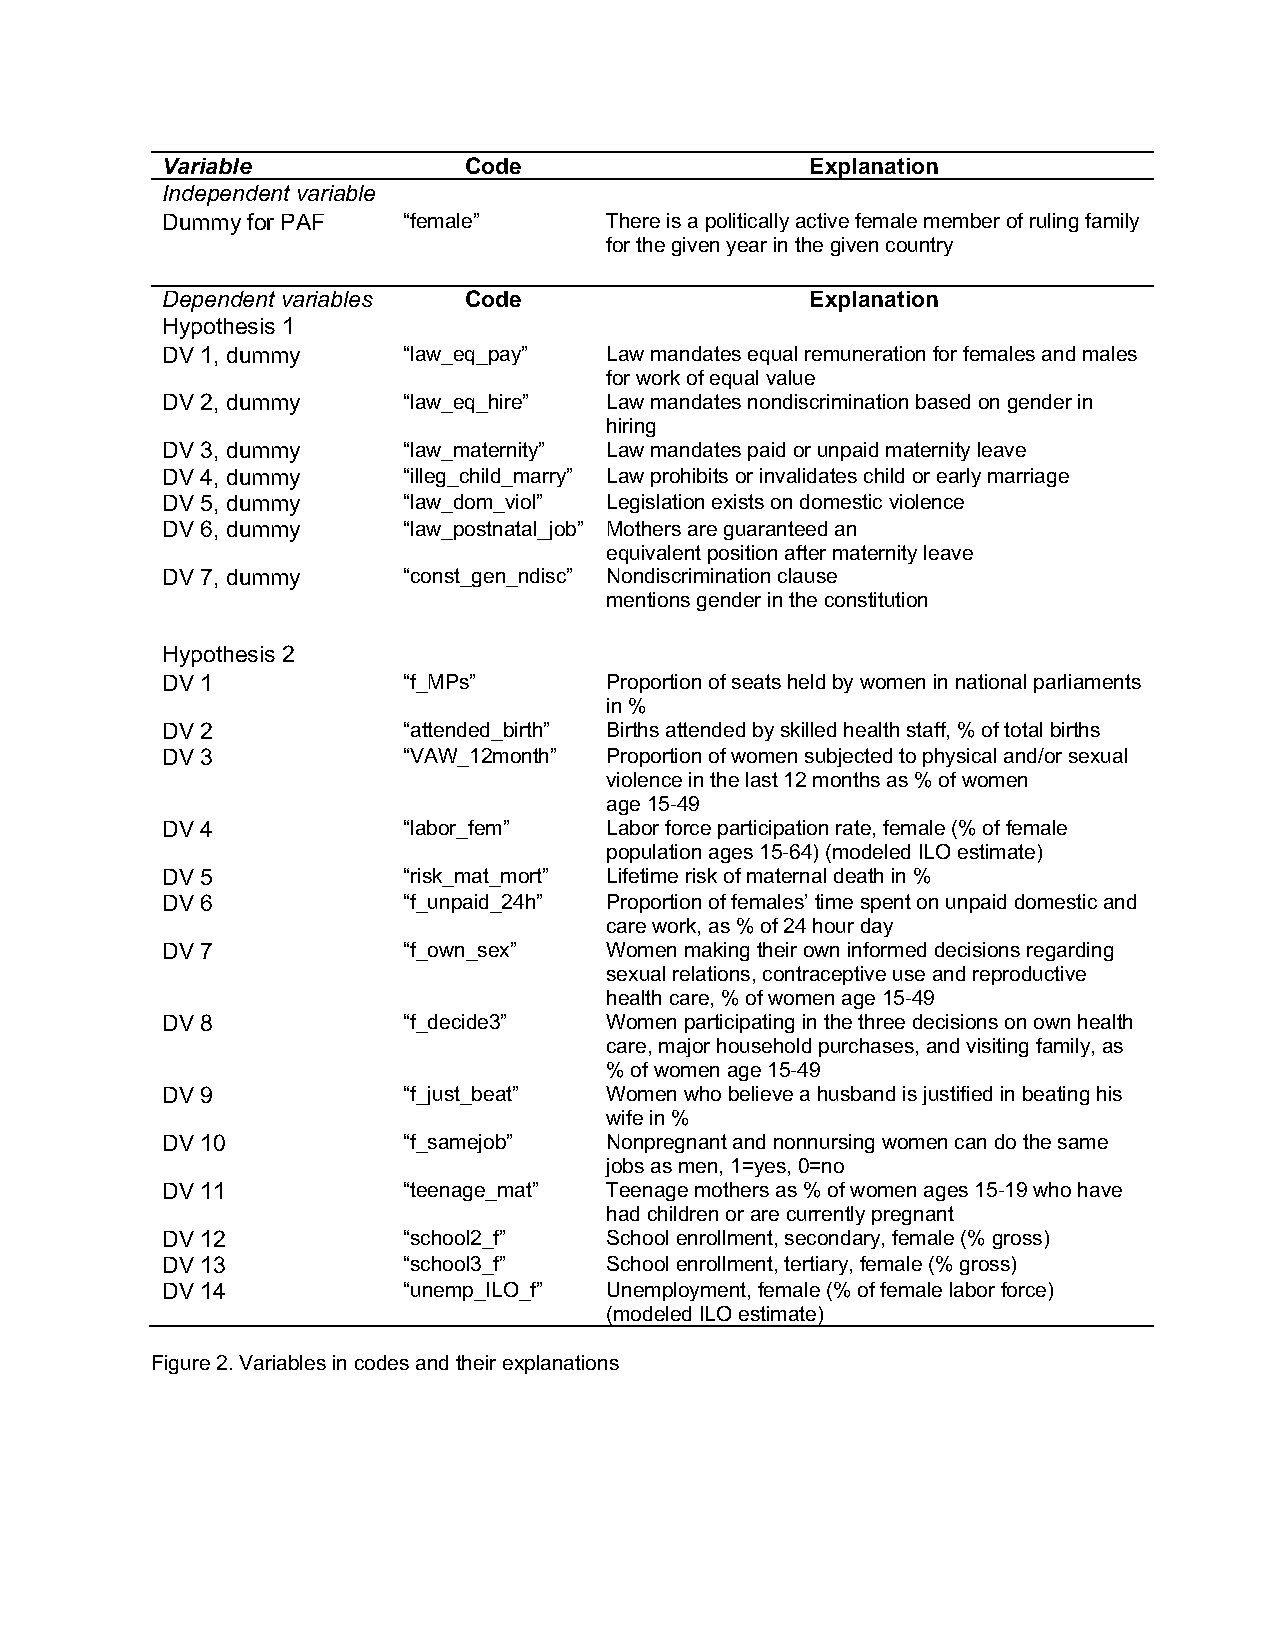
\includegraphics[width=16.5cm]{Variables.pdf}
\label{fig:}
\end{figure}

\section*{Data and Empirical Strategy}

The key independent variable employed is the presence of politically active female member of ruling family in a non-democracy (PAF) for each country in panel dataset in the given time period. To calculate the effect of pro-women legislation and policy outcomes, the formal notations of estimate is created as following:

\[ Law/Policy_{it} = \alpha + \beta female_{it} + \gamma X_{it} + \sigma_{i} + \theta_{t} + \epsilon_{it} \]
where $Law_{it}$ and $Policy_{it}$ represent pro-women legislation and policy outcomes respectively. \texttt{female} is a dummy variable for the presence of PAF. X is a set of controls that includes log GDP per capita, the share of agricultural cluster in the GDP, urban population as percent of total population, total debt servicing as share of GDP, and total funds spent on education as percent of GDP. $\sigma_{i}$ and $\theta_{t}$ are country and year fixed/random effects depending on the model used. And finally, $\epsilon_{it}$ is a normally distributed error term. $i$ indexes countries as sovereign political regimes and $t$ indexes time. Standard errors are clustered by country-year. The estimate of interest is $\beta$, the effect of changes in the presence of \texttt{female} on changes in pro-women legislation and policies. 

I obtained my data sources on regime variation from the Polity IV dataset. For political family composition, I surveyed Wikipedia profiles of ruling families, at least one reputed newspaper that covers a country of each ruling family, and official biographies whenever available. My units of analysis for this research are countries and years that contain at least two non-democratic regime periods. For this, I created a dummy variable \texttt{polity4} which gets a value of 1 if a country-year is democratic and 0 if non-democratic. To be coded as non-democratic in a year-period, countries should obtain scores 5 or lower, and be labelled by Polity IV as either anocracy (open or closed) or authoritarian. 

There are 69 countries in my panel dataset. Countries that did not have at least two non-democratic regime periods as coded by Polity IV for years 2000-2019 are not included in my panel data. There are two notable cases among non-democracies. First, Myanmar is not included in the dataset, because its statistical reporting is periodically more scarce than even that of North Korea's. Second, Ecuador is included because its last two years in the dataset correspond to non-democratic criteria, although it will not suffice a typical non-democratic profile in other periods. Some countries may have  periods with both regime labels. For example, Georgia had an authoritarian period under Shevarnadze until 2003, but is democratic now. In contrast, Kazakhstan maintained non-democratic regime evenly after political transition and therefore all periods for \texttt{polity4} get 0. 
 
For the outcome variables on two hypotheses, I derived all my data from the World Bank's Global Development Indicators for 20 years, from 2000 to 2019. The reason for considering the time period of 2000-2019 is straightforward: World Bank started collecting data on most outcomes of interest from 2000, as part of the Millennium and now Sustainable Development Goals. In future extensions of this work, more qualitative work is needed to consult national legal frameworks of all 69 countries from this panel dataset to fill the missing entries on pro-women laws. Where needed, pro-women policy outcome entries with missing data can be filled consulting national statistical publications and development economics literature. Both should help to increase the power of employed models in future extensions. 

Using this strategy, the causal directionality effects of changes in the presence of PAF is statistically identified using pooled OLS and random country effects from the \texttt{plm package in R} (panel linear regression). 

\section*{Evidence and Robustness Checks}

\textbf{N.B.:} \textit{All tables with coefficients of interest and p-values with model specification and standard errors can be found in tables 1 to 8 after the }\textbf{Conclusion} \textit{section of this paper. Full models with complete data, all codes, and visualizations can be found in Appendix.} 

Recalling the earlier discussion, I ran my pooled OLS model for panel data on both hypotheses. I then employed random and fixed effects extensions for hypotheses 1 and 2 models, respectively. For the sake of parsimony, I report in this paper only statistically significant model estimates, clearly stating their origins. Full models with all summary tables and visualizations can be found in Appendix. 

There is a characteristic issue with the exogeneity of independent variable \texttt{female}. I employ a number of theoretically motivated control variables for both hypotheses, as discussed in the previous section, and introduce an interaction variable of \texttt{postcommunism} when estimating outcome variables for hypothesis 2. The use of pooled OLS for both hypotheses as a baseline model is validated by Breusch-Pagan Lagrange multiplier (LM) test and robust for cross-sectional dependence-contemporaneous correlation using Breusch-Pagan LM test of independence and Pasaran CD test (see Appendix). $R^2$ of all reported pooled OLS models are robust. Nevertheless, this research's first model of pooled OLS should be treated as exploratory and its methods as observational, albeit pointing toward promising causal story. 

\textbf{For outcomes of interest on hypothesis 1}, only two legislation pieces came with statistically significant results, hence rejecting null hypothesis in two out of seven outcomes of interest. One outcome of interest detected statistically significant effects for controls only (gender non-discrimination clause in the constitution). Although interesting, law on domestic violence is negatively correlated with the independent variable at 0.01 statistical significance, pointing at opposite direction. One standard deviation increase in the presence of PAF leads to almost 17 standard deviation decrease in the country having a law on domestic violence. Thus, in line with my hypothesis, null was rejected for: (1) prohibition of child marriage and (3) guaranteed post-maternity leave job of equivalent position prior to taking the leave, with 0.1 and 0.01 statistical significance only. 

Then, to determine whether to employ fixed or random effect estimators for hypothesis 1's model extension, I conducted a Hausman test, which tests whether the unique errors are correlated with the regressors (the null is they are not). Since Hausman test p-values were not significant, pointing that the unique errors were not correlated with the regressors, I chose random effects extension to test hypothesis 1. In line with the requirements for transparency and integrity, I provide estimates for hypothesis 1 year and country fixed-effects as well in Appendix. In the extension model, none of the two rejected null outcomes of interest maintained statistical significance. In two of four models, random effects resulted in aborted observations, likely due to the limited number of observations at year level. Figures 1 and 2 that are placed after the \textbf{Conclusion} section show that the year-level variation is limited for both of those models. Overall, none of the pro-women laws out of seven selected, or 100\% of cases, saw any positive correlation with the presence of PAF in non-democracies under random effects. 

\textbf{For outcomes of interest on hypothesis 2}, I hypothesized that the presence of PAF would not result in pro-women policy outcomes. Recall that I theoretically motivated this hypothesis with the nature of non-democracy, where it is easy to make ``cheap-talk" by passing legislation, but much more difficult to implement policies. The latter is especially true when non-democratic countries are plagued with weak state capacity, corruption, and the lack of accountability. Therefore, absent statistically significant effects point to the absence of such relationship. Dependent variables for hypothesis 2 are supported with more coherent data, available with significant cross-country and year variations. Descriptive visualization of this can be seen in Figures 3 and 4 that come after the \textbf{Conclusion} section. 

To test for hypothesis 2, I first ran 14 OLS pooled regressions with control variables and interaction on postcommunist legacy. For postcommunist legacy, I coded countries with active communist regimes (e.g. China, Cuba, North Korea, Lao, and Vietnam) or recent communist past (e.g. Gabon or Tajikistan), the cutoff year for the latter being the collapse of the USSR in 1991. All pooled OLS models but one are robust to validation by Breusch-Pagan Lagrange multiplier (LM) test, and all 14 are robust for cross-sectional dependence-contemporaneous correlation using Breusch-Pagan LM test of independence and Pasaran CD test (see Appendix). Of 14 pooled OLS models, 11 did not have statistically significant effects, rejecting the null hypothesis that the presence of PAF had positive effect on pro-women policy outcomes. Only three models failed to reject null hypothesis. At closer examination of Tables 5 to 7 that can be found after the \textbf{Conclusion} section, we see that the independent variable has statistically significant effect on three policy outcomes: the lifetime risk of maternal mortality, female laborforce participation, and births attended by skilled professionals all at 0.01 statistical significance level. In fact, the latter has opposite directionality, with one standard deviation increase in PAF presence resulting in drastic 7.86 standard deviations decrease in births attended by skilled professionals.  

The dependent variable of women justifying beating by a husband due to any of the five surveyed reasons had initially recorded statistical significance, but the estimate was not robust to Breusch-Pagan Lagrange multiplier (LM) test, suggesting random country correlation. Therefore, I retested justification of beating through random country effect extension which resulted in null effect. I report this case in Table 8, which also includes fixed effect extension. 

Finally, I extended three pooled OLS models where null is rejected with Year and country specific fixed effects in a two-ways model. Robustness checks for fixed effect on cross-sectional dependence and contemporaneous correlation were conducted using Breusch-Pagan LM test of independence and Pasaran CD test. No cross-sectional dependence was detected. Thanks to a combination of control variables, interaction term, and two-ways fixed effects, the variation in the PAF that remained was more likely not to be endogenous to country and year-specific shocks. After applying fixed effects, all but one statistically significant estimate disappeared. Female laborforce participation had positive relationship with PAF presence and was robust to fixed effects at 0.01 significance level, although negatively correlated when interacted with postcommunism. Overall, 13 out of 14 pro-women policy outcomes of interest did not see positive effect due to the presence of PAF in a non-democracy, thus rejecting the null hypothesis at 93\% of cases. 

As it occurs, the mere increase of elite descriptive representation for women in non-democracies did not result in pro-women legislation (proclamations) or policies (actions). Democratic power authorization and resultant accountability seem to be reinforced as important conditions if substantive representation of women in non-democratic regime periods is to be achieved. 

\section*{Conclusion}
Through implementing pooled OLS tests with relevant fixed or random effects, control variables, interaction term, and robustness checks I find that, in correspondence with my hypothesis 1, the presence of PAF has weak positive effect only on a small subset of predefined pro-women legislative outcomes, but it mostly disappears under fixed and random effects. In line with the theoretical motivation for my hypothesis 2, the presence of PAF has no statistically discernible positive effect on 13 out of 14 predefined pro-women policy outcomes, even after case countries are interacted with postcommunism variable. This exploratory analysis of data weakly supports an alternative explanation that there are no popular benefits from the mere increase of descriptive and symbolic representation in non-democracies. Democratic authorization and accountability may be much more important than descriptive representation. This research is useful in its exploration of relationship between non-democratic regimes and the concepts of political representation. Future extensions of this work should consider longer time-span and more complete country-level inputs for variables.

%FIGURE 2
\begin{figure}[!htbp]
\centering
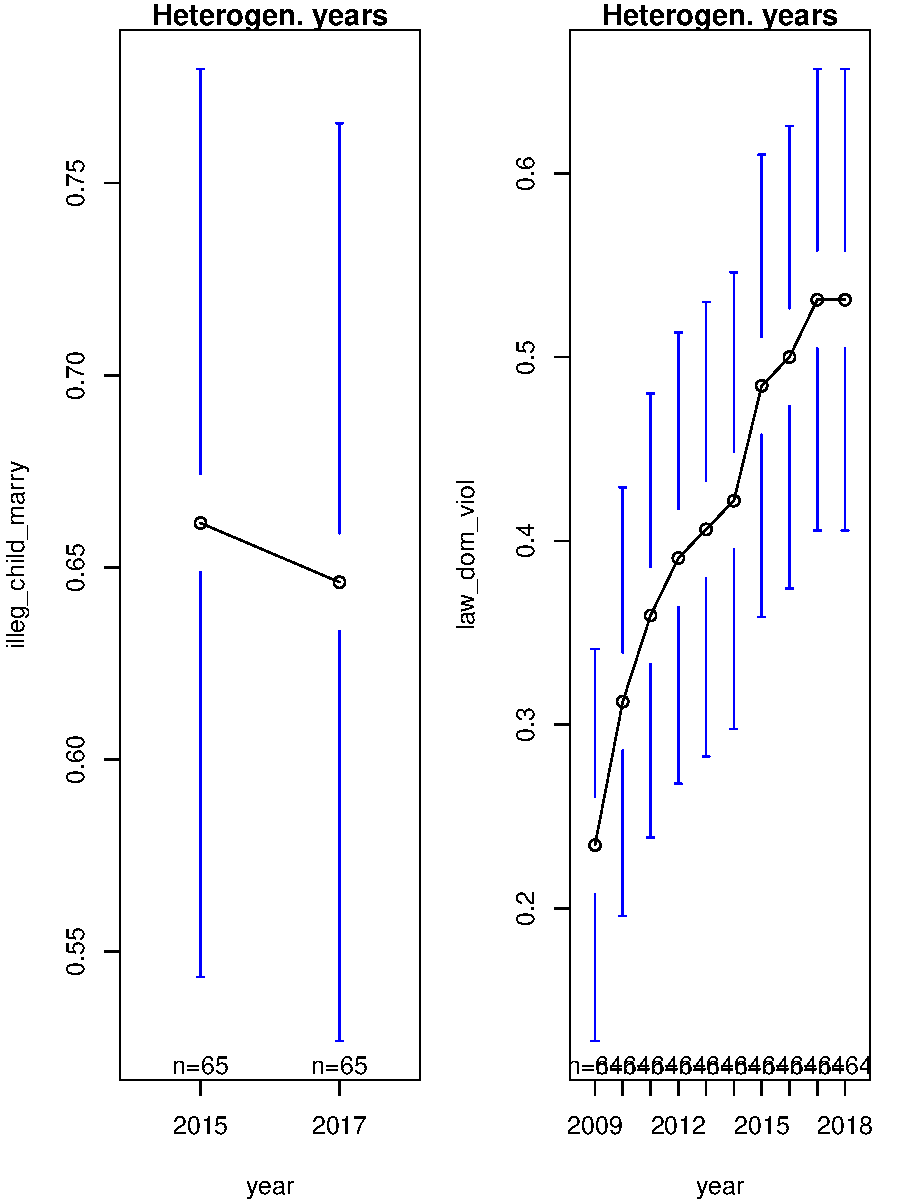
\includegraphics[width=16cm]{Plot1.pdf}
\caption{Hypothesis 1, DV 4 and 5}
\label{fig:hypothesis 1 1-2}
\end{figure}


%FIGURE 3
\begin{figure}[htp]
\centering
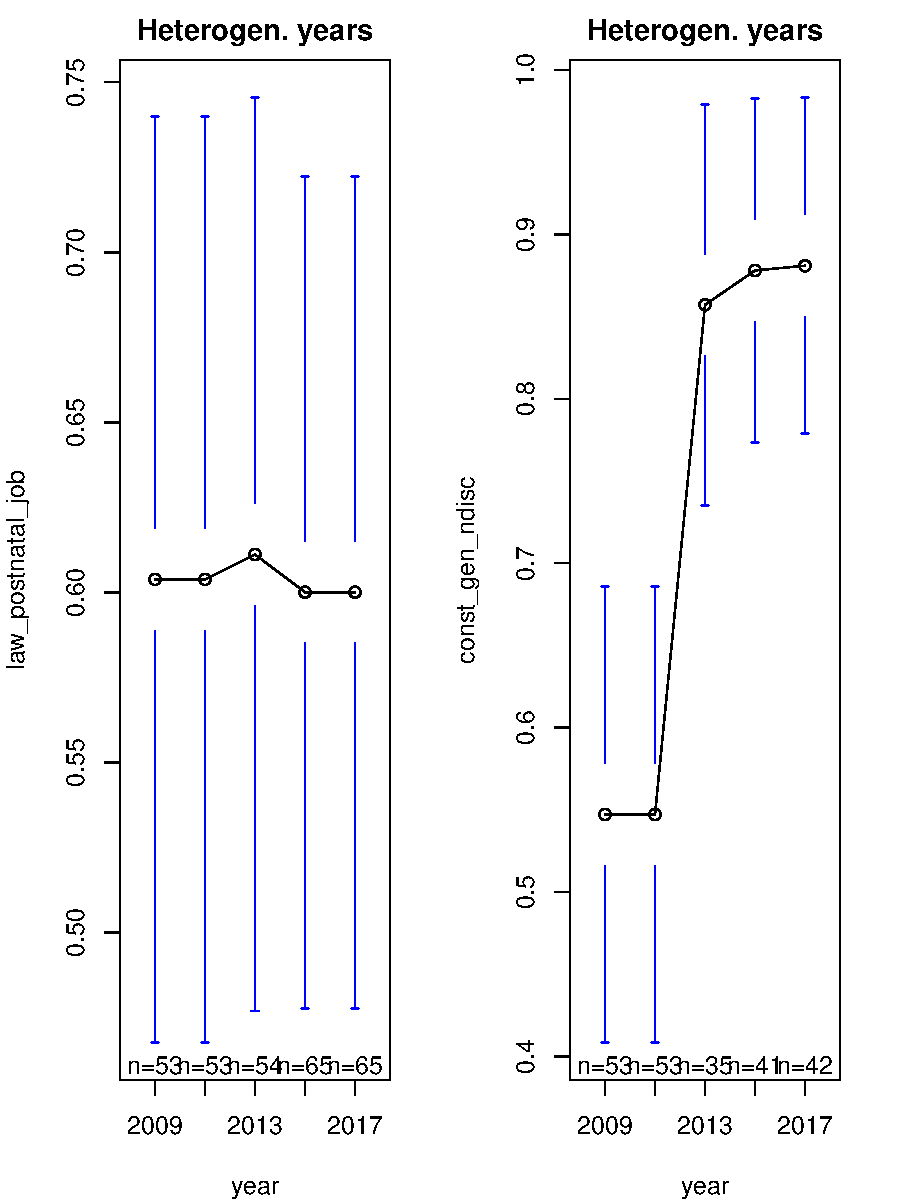
\includegraphics[width=16cm]{Plot2.pdf}
\caption{Hypothesis 1, DV 6 and 7}
\label{fig:hypothesis 1 3-4}
\end{figure}

% H1 - outcome 1
\begin{table}[!htbp] 
\centering 
  \caption{Hypothesis 1, outcome 1} 
  \label{} 
\begin{tabular}{@{\extracolsep{5pt}}lcc} 
\\[-1.8ex]\hline 
\hline \\[-1.8ex] 
 & \multicolumn{2}{c}{\textit{Dependent variable:}} \\ 
\cline{2-3} 
\\[-1.8ex] & \multicolumn{2}{c}{Prohibited child/early marriage} \\ 
\\[-1.8ex] & (Pooled OLS) & (Random-effect, country)\\ 
\hline \\[-1.8ex] 
 female & 0.231$^{*}$ &  \\ 
  & (0.114) &  \\ 
  & & \\ 
 log(gdp\_pc) & 0.021 & 0.000 \\ 
  & (0.117) & (0.000) \\ 
  & & \\ 
 agric\_share & $-$0.004 & 0.000 \\ 
  & (0.009) & (0.000) \\ 
  & & \\ 
 urban\_pop & $-$0.006 & 0.000 \\ 
  & (0.005) & (0.000) \\ 
  & & \\ 
 debt\_service & 0.031$^{**}$ & 0.000 \\ 
  & (0.013) & (0.000) \\ 
  & & \\ 
 edu\_gdp & 0.158$^{***}$ & 0.000 \\ 
  & (0.040) & (0.000) \\ 
  & & \\ 
 Constant & 0.060 &  \\ 
  & (0.792) &  \\ 
  & & \\ 
\hline \\[-1.8ex] 
Observations & 44 & 44 \\ 
R$^{2}$ & 0.453 &  \\ 
Adjusted R$^{2}$ & 0.364 &  \\ 
F Statistic & 5.102$^{***}$ (df = 6; 37) &  \\ 
\hline 
\hline \\[-1.8ex] 
\textit{Note:}  & \multicolumn{2}{r}{$^{*}$p$<$0.1; $^{**}$p$<$0.05; $^{***}$p$<$0.01} \\ 
\end{tabular} 
\end{table} 



% H1 - outcome 2
\begin{table}[!htbp] \centering 
  \caption{Hypothesis 1, outcome 2} 
  \label{} 
\begin{tabular}{@{\extracolsep{5pt}}lcc} 
\\[-1.8ex]\hline 
\hline \\[-1.8ex] 
 & \multicolumn{2}{c}{\textit{Dependent variable:}} \\ 
\cline{2-3} 
\\[-1.8ex] & \multicolumn{2}{c}{Law on Domestic Violence} \\ 
\\[-1.8ex] & (Pooled OLS) & (Random-effect, country)\\ 
\hline \\[-1.8ex] 
 female & $-$0.170$^{***}$ & $-$0.180$^{**}$ \\ 
  & (0.057) & (0.086) \\ 
  & & \\ 
 log(gdp\_pc) & 0.101$^{**}$ & 0.105 \\ 
  & (0.051) & (0.097) \\ 
  & & \\ 
 agric\_share & $-$0.016$^{***}$ & $-$0.005 \\ 
  & (0.004) & (0.006) \\ 
  & & \\ 
 urban\_pop & $-$0.019$^{***}$ & $-$0.007 \\ 
  & (0.002) & (0.005) \\ 
  & & \\ 
 debt\_service & 0.035$^{***}$ & 0.012 \\ 
  & (0.007) & (0.008) \\ 
  & & \\ 
 edu\_gdp & 0.026 & $-$0.011 \\ 
  & (0.017) & (0.022) \\ 
  & & \\ 
 Constant & 0.668$^{*}$ & 0.120 \\ 
  & (0.376) & (0.672) \\ 
  & & \\ 
\hline \\[-1.8ex] 
Observations & 266 & 266 \\ 
R$^{2}$ & 0.290 & 0.038 \\ 
Adjusted R$^{2}$ & 0.273 & 0.016 \\ 
F Statistic & 17.612$^{***}$ (df = 6; 259) & 10.127 \\ 
\hline 
\hline \\[-1.8ex] 
\textit{Note:}  & \multicolumn{2}{r}{$^{*}$p$<$0.1; $^{**}$p$<$0.05; $^{***}$p$<$0.01} \\ 
\end{tabular} 
\end{table} 


% H1 - outcome 3
\begin{table}[!htbp] \centering 
  \caption{Hypothesis 1, outcome 3} 
  \label{} 
\begin{tabular}{@{\extracolsep{5pt}}lcc} 
\\[-1.8ex]\hline 
\hline \\[-1.8ex] 
 & \multicolumn{2}{c}{\textit{Dependent variable:}} \\ 
\cline{2-3} 
\\[-1.8ex] & \multicolumn{2}{c}{Job Guaranteed Post-Maternity Leave} \\ 
\\[-1.8ex] & (Pooled OLS) & (Random-effect, country)\\ 
\hline \\[-1.8ex] 
 female & 0.222$^{***}$ & 0.000 \\ 
  & (0.077) & (0.000) \\ 
  & & \\ 
 log(gdp\_pc) & 0.068 & 0.000 \\ 
  & (0.078) & (0.000) \\ 
  & & \\ 
 agric\_share & 0.012$^{**}$ & 0.000 \\ 
  & (0.005) & (0.000) \\ 
  & & \\ 
 urban\_pop & 0.007$^{*}$ & 0.000 \\ 
  & (0.004) & (0.000) \\ 
  & & \\ 
 debt\_service & $-$0.003 & 0.000 \\ 
  & (0.008) & (0.000) \\ 
  & & \\ 
 edu\_gdp & 0.042$^{*}$ & 0.000 \\ 
  & (0.024) & (0.000) \\ 
  & & \\ 
 Constant & $-$0.565 &  \\ 
  & (0.550) &  \\ 
  & & \\ 
\hline \\[-1.8ex] 
Observations & 132 & 132 \\ 
R$^{2}$ & 0.149 &  \\ 
Adjusted R$^{2}$ & 0.108 &  \\ 
F Statistic & 3.656$^{***}$ (df = 6; 125) &  \\ 
\hline 
\hline \\[-1.8ex] 
\textit{Note:}  & \multicolumn{2}{r}{$^{*}$p$<$0.1; $^{**}$p$<$0.05; $^{***}$p$<$0.01} \\ 
\end{tabular} 
\end{table}


% H1 - outcome 4
\begin{table}[!htbp] \centering 
  \caption{Hyptohesis 1, outcome 4} 
  \label{} 
\begin{tabular}{@{\extracolsep{5pt}}lcc} 
\\[-1.8ex]\hline 
\hline \\[-1.8ex] 
 & \multicolumn{2}{c}{\textit{Dependent variable:}} \\ 
\cline{2-3} 
\\[-1.8ex] & \multicolumn{2}{c}{Gender Non-discrimination in Constitution} \\ 
\\[-1.8ex] & (1) & (2)\\ 
\hline \\[-1.8ex] 
 female & $-$0.085 & $-$0.049 \\ 
  & (0.085) & (0.068) \\ 
  & & \\ 
 log(gdp\_pc) & 0.265$^{***}$ & 0.338$^{***}$ \\ 
  & (0.085) & (0.105) \\ 
  & & \\ 
 agric\_share & 0.011$^{**}$ & 0.007 \\ 
  & (0.005) & (0.005) \\ 
  & & \\ 
 urban\_pop & $-$0.018$^{***}$ & $-$0.019$^{***}$ \\ 
  & (0.004) & (0.006) \\ 
  & & \\ 
 debt\_service & 0.007 & 0.007 \\ 
  & (0.010) & (0.007) \\ 
  & & \\ 
 edu\_gdp & 0.051$^{**}$ & 0.063$^{***}$ \\ 
  & (0.025) & (0.022) \\ 
  & & \\ 
 Constant & $-$0.925 & $-$1.452$^{**}$ \\ 
  & (0.586) & (0.685) \\ 
  & & \\ 
\hline \\[-1.8ex] 
Observations & 105 & 105 \\ 
R$^{2}$ & 0.296 & 0.116 \\ 
Adjusted R$^{2}$ & 0.253 & 0.062 \\ 
F Statistic & 6.879$^{***}$ (df = 6; 98) & 12.121$^{*}$ \\ 
\hline 
\hline \\[-1.8ex] 
\textit{Note:}  & \multicolumn{2}{r}{$^{*}$p$<$0.1; $^{**}$p$<$0.05; $^{***}$p$<$0.01} \\ 
\end{tabular} 
\end{table}

%FIGURE 4
\begin{figure}[htp]
\centering
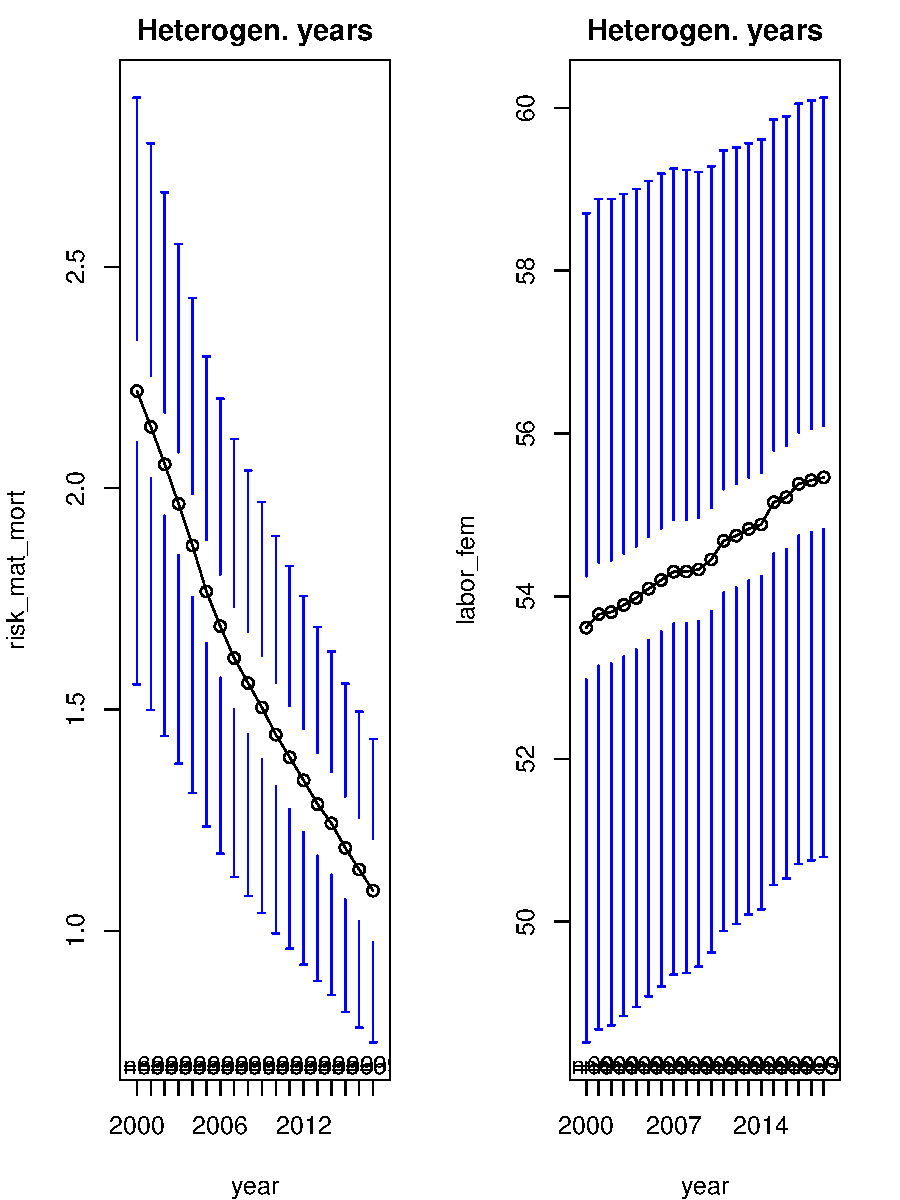
\includegraphics[width=16cm]{H2m3-9.pdf}
\caption{Hypothesis 2, DV 5 and 4}
\label{fig:hypothesis 1 1-2}
\end{figure}


%FIGURE 5
\begin{figure}[htp]
\centering
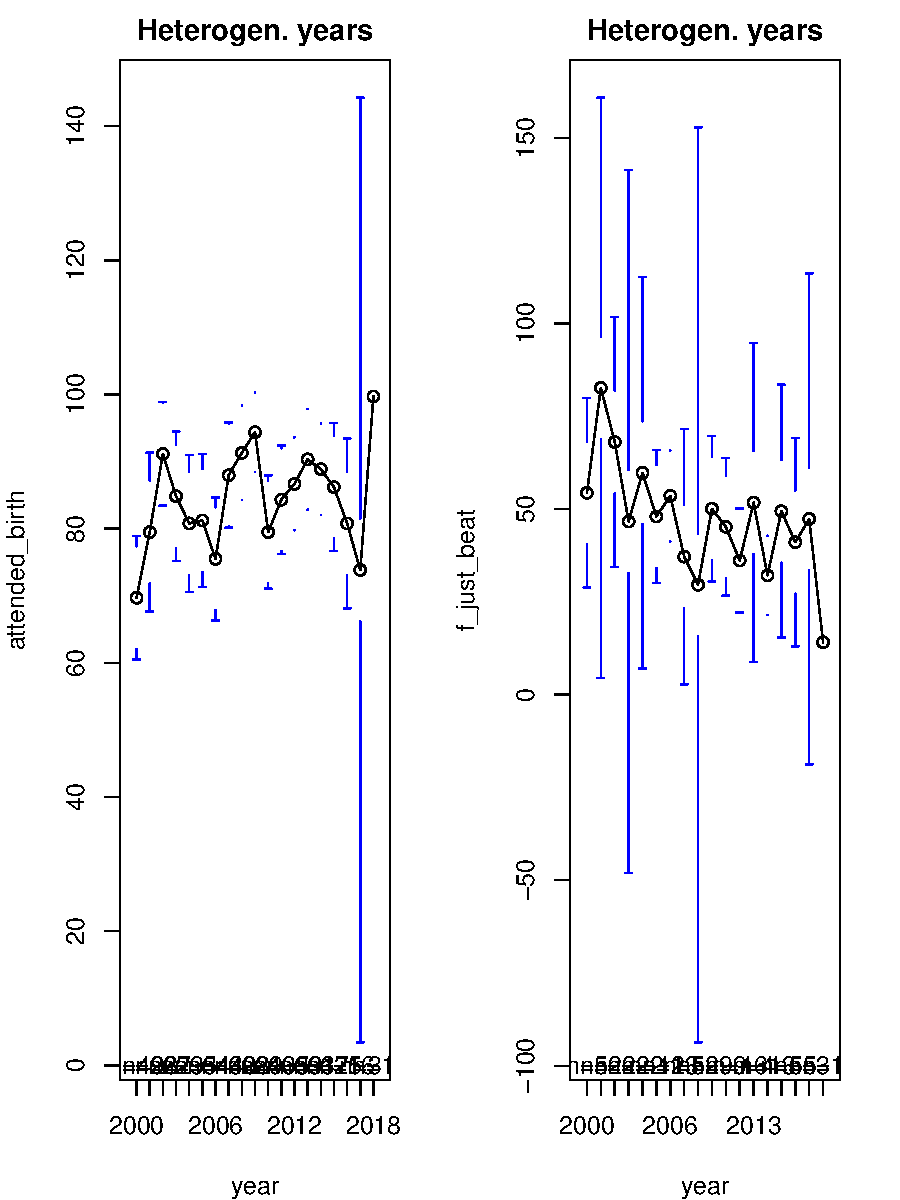
\includegraphics[width=16cm]{H2m15-7.pdf}
\caption{Hypothesis 2, DV 2 and 9}
\label{fig:hypothesis 1 3-4}
\end{figure}


% Hypothesis 2 Outcome 1
\begin{table}[!htbp] \centering 
  \caption{Hypothesis 2, Outcome 1} 
  \label{} 
\begin{tabular}{@{\extracolsep{5pt}}lcc} 
\\[-1.8ex]\hline 
\hline \\[-1.8ex] 
 & \multicolumn{2}{c}{\textit{Dependent variable:}} \\ 
\cline{2-3} 
\\[-1.8ex] & \multicolumn{2}{c}{Lifetime Rist of Maternal Mortality} \\ 
\\[-1.8ex] & (Pooled OLS) & (Fixed Effects)\\ 
\hline \\[-1.8ex] 
 female & 0.535$^{***}$ & $-$0.002 \\ 
  & (0.157) & (0.132) \\ 
  & & \\ 
 post\_com & $-$1.058$^{***}$ &  \\ 
  & (0.173) &  \\ 
  & & \\ 
 log(gdp\_pc) & $-$0.743$^{***}$ & 0.404$^{**}$ \\ 
  & (0.114) & (0.185) \\ 
  & & \\ 
 agric\_share & 0.071$^{***}$ & $-$0.017$^{**}$ \\ 
  & (0.009) & (0.007) \\ 
  & & \\ 
 urban\_pop & 0.020$^{***}$ & $-$0.011 \\ 
  & (0.005) & (0.015) \\ 
  & & \\ 
 debt\_service & 0.008 & 0.015 \\ 
  & (0.014) & (0.009) \\ 
  & & \\ 
 edu\_gdp & $-$0.224$^{***}$ & $-$0.048 \\ 
  & (0.040) & (0.031) \\ 
  & & \\ 
 female:post\_com & $-$1.105$^{***}$ &  \\ 
  & (0.239) &  \\ 
  & & \\ 
 Constant & 6.335$^{***}$ &  \\ 
  & (0.879) &  \\ 
  & & \\ 
\hline \\[-1.8ex] 
Observations & 525 & 525 \\ 
R$^{2}$ & 0.628 & 0.049 \\ 
Adjusted R$^{2}$ & 0.623 & $-$0.105 \\ 
F Statistic & 109.024$^{***}$ (df = 8; 516) & 3.873$^{***}$ (df = 6; 451) \\ 
\hline 
\hline \\[-1.8ex] 
\textit{Note:}  & \multicolumn{2}{r}{$^{*}$p$<$0.1; $^{**}$p$<$0.05; $^{***}$p$<$0.01} \\ 
\end{tabular} 
\end{table} 

% Hypothesis 2, Outcome 2
\begin{table}[!htbp] \centering 
  \caption{Hypothesis 2, Outcome 2} 
  \label{} 
\begin{tabular}{@{\extracolsep{5pt}}lcc} 
\\[-1.8ex]\hline 
\hline \\[-1.8ex] 
 & \multicolumn{2}{c}{\textit{Dependent variable:}} \\ 
\cline{2-3} 
\\[-1.8ex] & \multicolumn{2}{c}{Female Laborforce Participation} \\ 
\\[-1.8ex] & (Pooled OLS) & (Fixed Effects)\\ 
\hline \\[-1.8ex] 
 female & 7.675$^{***}$ & 6.472$^{***}$ \\ 
  & (1.958) & (2.000) \\ 
  & & \\ 
 post\_com & 21.613$^{***}$ &  \\ 
  & (2.164) &  \\ 
  & & \\ 
 log(gdp\_pc) & $-$3.633$^{**}$ & 2.653$^{***}$ \\ 
  & (1.418) & (0.735) \\ 
  & & \\ 
 agric\_share & 0.246$^{**}$ & 0.066$^{**}$ \\ 
  & (0.114) & (0.026) \\ 
  & & \\ 
 urban\_pop & $-$0.178$^{***}$ & 0.259$^{***}$ \\ 
  & (0.068) & (0.059) \\ 
  & & \\ 
 debt\_service & 0.499$^{***}$ & 0.190$^{***}$ \\ 
  & (0.174) & (0.036) \\ 
  & & \\ 
 edu\_gdp & $-$0.803 & $-$0.381$^{***}$ \\ 
  & (0.494) & (0.119) \\ 
  & & \\ 
 female:post\_com & $-$15.678$^{***}$ & $-$4.875$^{**}$ \\ 
  & (2.975) & (2.071) \\ 
  & & \\ 
 Constant & 79.703$^{***}$ &  \\ 
  & (10.964) &  \\ 
  & & \\ 
\hline \\[-1.8ex] 
Observations & 527 & 527 \\ 
R$^{2}$ & 0.290 & 0.211 \\ 
Adjusted R$^{2}$ & 0.279 & 0.080 \\ 
F Statistic & 26.495$^{***}$ (df = 8; 518) & 17.234$^{***}$ (df = 7; 451) \\ 
\hline 
\hline \\[-1.8ex] 
\textit{Note:}  & \multicolumn{2}{r}{$^{*}$p$<$0.1; $^{**}$p$<$0.05; $^{***}$p$<$0.01} \\ 
\end{tabular} 
\end{table} 

% Hypothesis 2, Outcome 3
\begin{table}[!htbp] \centering 
  \caption{Hypothesis 2, Outcome 3} 
  \label{} 
\begin{tabular}{@{\extracolsep{5pt}}lcc} 
\\[-1.8ex]\hline 
\hline \\[-1.8ex] 
 & \multicolumn{2}{c}{\textit{Dependent variable:}} \\ 
\cline{2-3} 
\\[-1.8ex] & \multicolumn{2}{c}{Births Attended Professionally} \\ 
\\[-1.8ex] & (Pooled OLS) & (Fixed Effects)\\ 
\hline \\[-1.8ex] 
 female & $-$7.860$^{***}$ & $-$0.446 \\ 
  & (2.983) & (2.569) \\ 
  & & \\ 
 post\_com & 0.387 &  \\ 
  & (2.882) &  \\ 
  & & \\ 
 log(gdp\_pc) & 5.823$^{***}$ & 7.156$^{*}$ \\ 
  & (2.142) & (4.149) \\ 
  & & \\ 
 agric\_share & $-$0.621$^{***}$ & $-$0.012 \\ 
  & (0.174) & (0.166) \\ 
  & & \\ 
 urban\_pop & 0.325$^{***}$ & 0.565 \\ 
  & (0.100) & (0.414) \\ 
  & & \\ 
 debt\_service & 0.258 & 0.011 \\ 
  & (0.196) & (0.205) \\ 
  & & \\ 
 edu\_gdp & 5.945$^{***}$ & 0.778 \\ 
  & (0.597) & (0.792) \\ 
  & & \\ 
 female:post\_com & 26.886$^{***}$ &  \\ 
  & (3.838) &  \\ 
  & & \\ 
 Constant & 0.644 &  \\ 
  & (16.759) &  \\ 
  & & \\ 
\hline \\[-1.8ex] 
Observations & 255 & 255 \\ 
R$^{2}$ & 0.750 & 0.021 \\ 
Adjusted R$^{2}$ & 0.742 & $-$0.316 \\ 
F Statistic & 92.233$^{***}$ (df = 8; 246) & 0.663 (df = 6; 189) \\ 
\hline 
\hline \\[-1.8ex] 
\textit{Note:}  & \multicolumn{2}{r}{$^{*}$p$<$0.1; $^{**}$p$<$0.05; $^{***}$p$<$0.01} \\ 
\end{tabular} 
\end{table} 

%Hypothesis 2, Outcome 4
\begin{table}[!htbp] \centering 
  \caption{Hypothesis 2, Outcome 4} 
  \label{} 
\begin{tabular}{@{\extracolsep{5pt}}lcc} 
\\[-1.8ex]\hline 
\hline \\[-1.8ex] 
 & \multicolumn{2}{c}{\textit{Dependent variable:}} \\ 
\cline{2-3} 
\\[-1.8ex] & \multicolumn{2}{c}{Women Justify Beating} \\ 
\\[-1.8ex] & (Random Effects) & (Fixed Effects)\\ 
\hline \\[-1.8ex] 
 female & $-$3.471 & 11.583 \\ 
  & (7.583) & (13.223) \\ 
  & & \\ 
 post\_com & $-$12.203 &  \\ 
  & (8.282) &  \\ 
  & & \\ 
 log(gdp\_pc) & $-$19.418$^{***}$ & $-$34.019 \\ 
  & (4.845) & (33.349) \\ 
  & & \\ 
 agric\_share & $-$0.505$^{*}$ & $-$1.680$^{*}$ \\ 
  & (0.289) & (0.531) \\ 
  & & \\ 
 urban\_pop & $-$0.101 & 3.302 \\ 
  & (0.224) & (1.929) \\ 
  & & \\ 
 debt\_service & $-$0.033 & 1.516 \\ 
  & (0.544) & (1.296) \\ 
  & & \\ 
 edu\_gdp & $-$3.819$^{***}$ & $-$5.191 \\ 
  & (1.403) & (3.180) \\ 
  & & \\ 
 female:post\_com & 2.762 &  \\ 
  & (9.286) &  \\ 
  & & \\ 
 Constant & 220.490$^{***}$ &  \\ 
  & (32.952) &  \\ 
  & & \\ 
\hline \\[-1.8ex] 
Observations & 60 & 60 \\ 
R$^{2}$ & 0.571 & 0.910 \\ 
Adjusted R$^{2}$ & 0.504 & $-$1.652 \\ 
F Statistic & 67.708$^{***}$ & 3.374 (df = 6; 2) \\ 
\hline 
\hline \\[-1.8ex] 
\textit{Note:}  & \multicolumn{2}{r}{$^{*}$p$<$0.1; $^{**}$p$<$0.05; $^{***}$p$<$0.01} \\ 
\end{tabular} 
\end{table} 

\pagebreak

\section*{References}

Aidt, Toke S., and Bianca Dallal. ``Female Voting Power: The Contribution of Women’s Suffrage to the Growth of Social Spending in Western Europe (1869–1960)." \textit{Public Choice} 134, no. 3-4 (2008): 391-417.

Cruz, Cesi, Julien Labonne, and Pablo Querubin. 2017. ``Politician Family Networks and Electoral Outcomes: Evidence from the Philippines." \textit{American Economic Review} 107 (10):3006- 37.

Pitkin, Hanna Fenichel. 1967. \textit{The Concept of Representation}. Berkeley: University of California. 

Tripp, Aili Mari. 2015. \textit{Women and power in post-conflict Africa}. New York: Cambridge University Press.

Tripp, Aili Mari. 2019. \textit{Seeking Legitimacy: Why Arab Autocracies Adopt Women's Rights}. New York: Cambridge University Press,.

Urbinati, Nadia, and Mark E. Warren. 2008. ``The Concept of Representation in Contemporary Democratic Theory." \textit{Annual Review of Political Science} 11:387-412.

\end{document}
